\documentclass[class=article, crop=false]{standalone}
\usepackage[margin=1in]{geometry}
\usepackage[linesnumbered,ruled,vlined]{algorithm2e}
\usepackage{amsfonts}
\usepackage{amsmath}
\usepackage{amssymb}
\usepackage{amsthm}
\usepackage{enumitem}
\usepackage{fancyhdr}
\usepackage{hyperref}
\usepackage{minted}
\usepackage{multicol}
\usepackage{pdfpages}
\usepackage{standalone}
\usepackage[many]{tcolorbox}
\usepackage{tikz-cd}
\usepackage{transparent}
\usepackage{xcolor}
% \tcbuselibrary{minted}

\author{Nathan Solomon}

\newcommand{\fig}[1]{
    \begin{center}
        \includegraphics[width=\textwidth]{#1}
    \end{center}
}

% Math commands
\renewcommand{\d}{\mathrm{d}}
\DeclareMathOperator{\id}{id}
\DeclareMathOperator{\im}{im}
\DeclareMathOperator{\proj}{proj}
\DeclareMathOperator{\Span}{span}
\DeclareMathOperator{\Tr}{Tr}
\DeclareMathOperator{\tr}{tr}
\DeclareMathOperator{\ad}{ad}
\DeclareMathOperator{\ord}{ord}
%%%%%%%%%%%%%%% \DeclareMathOperator{\sgn}{sgn}
\DeclareMathOperator{\Aut}{Aut}
\DeclareMathOperator{\Inn}{Inn}
\DeclareMathOperator{\Out}{Out}
\DeclareMathOperator{\stab}{stab}

\newcommand{\N}{\ensuremath{\mathbb{N}}}
\newcommand{\Z}{\ensuremath{\mathbb{Z}}}
\newcommand{\Q}{\ensuremath{\mathbb{Q}}}
\newcommand{\R}{\ensuremath{\mathbb{R}}}
\newcommand{\C}{\ensuremath{\mathbb{C}}}
\renewcommand{\H}{\ensuremath{\mathbb{H}}}
\newcommand{\F}{\ensuremath{\mathbb{F}}}

\newcommand{\E}{\ensuremath{\mathbb{E}}}
\renewcommand{\P}{\ensuremath{\mathbb{P}}}

\newcommand{\es}{\ensuremath{\varnothing}}
\newcommand{\inv}{\ensuremath{^{-1}}}
\newcommand{\eps}{\ensuremath{\varepsilon}}
\newcommand{\del}{\ensuremath{\partial}}
\renewcommand{\a}{\ensuremath{\alpha}}

\newcommand{\abs}[1]{\ensuremath{\left\lvert #1 \right\rvert}}
\newcommand{\norm}[1]{\ensuremath{\left\lVert #1\right\rVert}}
\newcommand{\mean}[1]{\ensuremath{\left\langle #1 \right\rangle}}
\newcommand{\floor}[1]{\ensuremath{\left\lfloor #1 \right\rfloor}}
\newcommand{\ceil}[1]{\ensuremath{\left\lceil #1 \right\rceil}}
\newcommand{\bra}[1]{\ensuremath{\left\langle #1 \right\rvert}}
\newcommand{\ket}[1]{\ensuremath{\left\lvert #1 \right\rangle}}
\newcommand{\braket}[2]{\ensuremath{\left.\left\langle #1\right\vert #2 \right\rangle}}

\newcommand{\catname}[1]{{\normalfont\textbf{#1}}}

\newcommand{\up}{\ensuremath{\uparrow}}
\newcommand{\down}{\ensuremath{\downarrow}}

% Custom environments
\newtheorem{thm}{Theorem}[section]

\definecolor{probBackgroundColor}{RGB}{250,240,240}
\definecolor{probAccentColor}{RGB}{140,40,0}
\newenvironment{prob}{
    \stepcounter{thm}
    \begin{tcolorbox}[
        boxrule=1pt,
        sharp corners,
        colback=probBackgroundColor,
        colframe=probAccentColor,
        borderline west={4pt}{0pt}{probAccentColor},
        breakable
    ]
    \color{probAccentColor}\textbf{Problem \thethm.} \color{black}
} {
    \end{tcolorbox}
}

\definecolor{exampleBackgroundColor}{RGB}{212,232,246}
\newenvironment{example}{
    \stepcounter{thm}
    \begin{tcolorbox}[
      boxrule=1pt,
      sharp corners,
      colback=exampleBackgroundColor,
      breakable
    ]
    \textbf{Example \thethm.}
} {
    \end{tcolorbox}
}

\definecolor{propBackgroundColor}{RGB}{255,245,220}
\definecolor{propAccentColor}{RGB}{150,100,0}
\newenvironment{prop}{
    \stepcounter{thm}
    \begin{tcolorbox}[
        boxrule=1pt,
        sharp corners,
        colback=propBackgroundColor,
        colframe=propAccentColor,
        breakable
    ]
    \color{propAccentColor}\textbf{Proposition \thethm. }\color{black}
} {
    \end{tcolorbox}
}

\definecolor{thmBackgroundColor}{RGB}{235,225,245}
\definecolor{thmAccentColor}{RGB}{50,0,100}
\renewenvironment{thm}{
    \stepcounter{thm}
    \begin{tcolorbox}[
        boxrule=1pt,
        sharp corners,
        colback=thmBackgroundColor,
        colframe=thmAccentColor,
        breakable
    ]
    \color{thmAccentColor}\textbf{Theorem \thethm. }\color{black}
} {
    \end{tcolorbox}
}

\definecolor{corBackgroundColor}{RGB}{240,250,250}
\definecolor{corAccentColor}{RGB}{50,100,100}
\newenvironment{cor}{
    \stepcounter{thm}
    \begin{tcolorbox}[
        enhanced,
        boxrule=0pt,
        frame hidden,
        sharp corners,
        colback=corBackgroundColor,
        borderline west={4pt}{0pt}{corAccentColor},
        breakable
    ]
    \color{corAccentColor}\textbf{Corollary \thethm. }\color{black}
} {
    \end{tcolorbox}
}

\definecolor{lemBackgroundColor}{RGB}{255,245,235}
\definecolor{lemAccentColor}{RGB}{250,125,0}
\newenvironment{lem}{
    \stepcounter{thm}
    \begin{tcolorbox}[
        enhanced,
        boxrule=0pt,
        frame hidden,
        sharp corners,
        colback=lemBackgroundColor,
        borderline west={4pt}{0pt}{lemAccentColor},
        breakable
    ]
    \color{lemAccentColor}\textbf{Lemma \thethm. }\color{black}
} {
    \end{tcolorbox}
}

\definecolor{proofBackgroundColor}{RGB}{255,255,255}
\definecolor{proofAccentColor}{RGB}{80,80,80}
\renewenvironment{proof}{
    \begin{tcolorbox}[
        enhanced,
        boxrule=1pt,
        sharp corners,
        colback=proofBackgroundColor,
        colframe=proofAccentColor,
        borderline west={4pt}{0pt}{proofAccentColor},
        breakable
    ]
    \color{proofAccentColor}\emph{\textbf{Proof. }}\color{black}
} {
    \qed \end{tcolorbox}
}

\definecolor{noteBackgroundColor}{RGB}{240,250,240}
\definecolor{noteAccentColor}{RGB}{30,130,30}
\newenvironment{note}{
    \begin{tcolorbox}[
        enhanced,
        boxrule=0pt,
        frame hidden,
        sharp corners,
        colback=noteBackgroundColor,
        borderline west={4pt}{0pt}{noteAccentColor},
        breakable
    ]
    \color{noteAccentColor}\textbf{Note. }\color{black}
} {
    \end{tcolorbox}
}


\fancyhf{}
\lhead{Nathan Solomon}
\rhead{Page \thepage}
\pagestyle{fancy}

\begin{document}
\section{5/21/2024 lecture}
The history of Mars is split into three eras:
\begin{itemize}
    \item \textbf{Noachian:} Heavy asteroid bombardment \& active volcanos
    \item \textbf{Hesperian:} Lots of water and sulfer dioxide rain
    \item \textbf{Amazonian:} No atmosphere, weathering and oxidation has turned the surface red (from ferrous oxides) and flat/smooth
\end{itemize}
Habitable zone: the range of distances from a star at which liquid water could possibly exist on a planet. This changes over time, since stars get brighter as they age due to increasing pressure (helium is denser, so the gravity becomes stronger). For example, if life existed on Mars, it would've been only for 500 million years after the formation of the solar system. Evidence of water on Mars would also be evidence that Mars used to have an atmosphere, because that is the only way it could have been in the habitable zone.
\par
More massive stars have larger habitable zones, but shorter lifetimes. Towards the end of their lifespans, they get dimmer because they run out of fuel.
\par
Life can exist outside of the habitable zone of a star, so long as there is some source of heat. In fact, having a planet or moon doesn't need to be part of any solar system in order to support life.
\par
Europa, Enceladus, and other moons of Jovian planets are good candidates for finding life. That's because tidal heating can be a significant source of heat. Tidal heating is especially notable on Io. This is because Io has an eccentric orbit, and it is closer to Jupiter than the other Galilean moons, so when it gets to perihelion, the gravitational field causes spagghetification, and the repeated deformation of Io heats it up via internal friction.
\par
The medium and large moons of Jovian planets are spherical (from self gravity) and orbit in the same direction as their planets, so they likely formed by accretion. A lot of the smaller moons appear to be captured asteroids, since they rotate the other way.
\par
Out of all of Jupiter's satellites, there are 4 moons which account for 
Europa has an extremely smooth surface. We think the orange spots on Europa could be from organic matter (specifically, tholin, which is a bunch of organic compounds made by ultraviolet irradiation of carbon compounds like methane), but that's just a guess. Studying Europa is hard because the radiation from Jupiter can damage a probe, so we would prefer to do a quick flyby.
\fig{tholin.jpg}
\par
There are two reasons we think Europa has a big salty subsurface ocean: we know from measurements of magnetic fields that Europa behaves as a conductor, and the scratch-like patterns (called stress fractures) look like ice, because we know ice is easier to deform than most other kinds of rocks.
\par
The main problems with Europa are the lack of nutrients and the high pressure at the bottom of the oceans.
\fig{Relative_Masses_of_Jovian_Satellites.png}
Ganymede and Callisto are both large and icy and probably have subsurface oceans. Ganymede has a magnetic field, but we don't consider it a major candidate for life because because the pressure in the subsurface oceans would be too high.
\par
Titan is the largest moon of Saturn. The surface has liquid methane and ethane which rain down, and also has enough of an atmosphere that we could fly there.
\par
We have sent a probe to land on the surface of Titan and taken pictures, which are shown below. There is a liquid lake on Titan, and we have pictures of river-like structures that resemble tributaries (although unfortunately they aren't water rivers). It's very very awesome that we have landed there, taken pictures, and found liquid lakes, but it is very cold (around 70 Kelvin) and doesn't seem to have the right chemicals to support life.
\begin{center}
    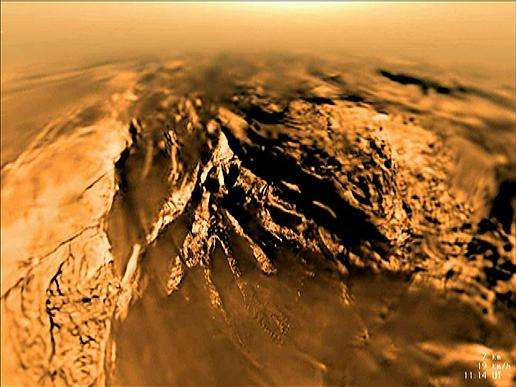
\includegraphics[width=.8\textwidth]{titan1.jpg}
\end{center}
\bigskip
\begin{center}
    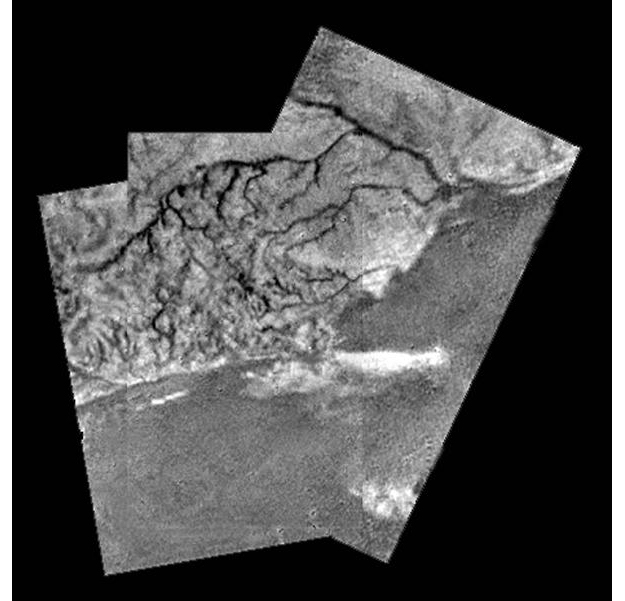
\includegraphics[width=.6\textwidth]{titan2.jpg}
\end{center}
\fig{titan3.png}
\par
Saturn's moon Enceladus is fairly small, but very interesting because it spews out plumes of warm water containing silica, salts, and phosphorus. The plumes are right above the bluish ``tiger stripes" on the surface.
\subsection{Water on Venus}
On Earth, most of the carbon and water are in the oceans (or somewhere other than the atmosphere). On Venus, those contribute to a very significant greenhouse effect.

\end{document}
